\secnumbersection{DEFINICIÓN DEL PROBLEMA}

\subsection{Contexto del problema}

La física computacional es un área multidisciplinaria cuyo objetivo es el desarrollo de modelos que permitan caracterizar fenómenos físicos derivados de las interacciones entre partículas, así como, crear métodos computacionales que nos permitan estudiar y generar predicciones del comportamiento de estas. Para el presente proyecto, únicamente consideraremos las áreas de la materia condensada, la física del estado sólido y la química.

Uno de los desafíos que se presentan en la investigación de estas estructuras radica en la cantidad de niveles de libertad que están pueden tener. Considerando que la materia está compuesta por muchas partículas (electrones, protones y neutrones), el tener en cuenta todas las posibles interacciones se vuelve una tarea muy difícil. Esto puede observarse en la siguiente expresión, que engloba las interacciones electrostáticas no relativistas entre partículas.

\begin{equation*}
    \mathcal{H} = -\sum_{i=!}^{N}\frac{1}{2}\nabla_i^2 - \sum_{A = 1}^{M} \frac{1}{2M_A}\nabla_A^{2} -\sum_{i=1}^{N}\sum_{A = 1}^{M} \frac{Z_A}{r_{iA}} + \sum_{i=1}^{N}\sum_{j>i}^{N} \frac{1}{r_{ij}}  + \sum_{A=1}^{M}\sum_{B>A}^{M} \frac{Z_AZ_B}{R_{AB}}
\end{equation*}

Frente a este dilema es que, teóricamente, se han propuesto diferentes aproximaciones que, bajo ciertos supuestos, permiten despreciar términos y tratar otros como valores constantes, reduciendo así las expresiones y los grados de libertad.

Una de las aproximaciones más famosa es la aproximación de Born-Oppenheimer\cite{BornOppenheimer}. Dado el modelo molecular de interacciones electrostáticas, si tomamos en cuenta la diferencia entre la energía cinética de los electrones frente al núcleo, es posible reducir la expresión original a la siguiente:

\begin{equation*}
    \mathcal{H}_{elec} = -\sum_{i=!}^{N}\frac{1}{2}\nabla_i^2  -\sum_{i=1}^{N}\sum_{A = 1}^{M} \frac{Z_A}{r_{iA}} + \sum_{i=1}^{N}\sum_{j>i}^{N} \frac{1}{r_{ij}}
\end{equation*}

El problema de este tipo de aproximaciones es que, a pesar de que se reduce el número de interacciones y grados de libertad, a medida que se tengan estructuras más complejas, el número de partículas sigue siendo muy grande (seguimos teniendo un problema de muchos cuerpos). De estas aproximaciones teóricas es que surgen los diversos hamiltonianos, los cuales son modelos que se enfocan en interacciones concretas, todos estos modelos son construidos en representaciones matriciales. Lamentablemente, estos siguen teniendo problemas de crecimiento a medida que se aumenta el número de partículas.

Para ejemplificar esto, consideremos un sistema de espines (el cual solo toma en cuenta las interacciones de los espines), que son representados como sumas de productos tensoriales de matrices cuadradas (matrices de Pauli), que tienen dimensión $(2S+1)^{2n}$ (siendo $n$ el tamaño del sistema y $S$ el espín). En la figura \ref{fig:1000} se puede apreciar los requerimientos de memoria RAM para mantener ese tipo de hamiltoniano en memoria, teniendo en cuenta diversos espines.


\begin{figure}[H]
\centering
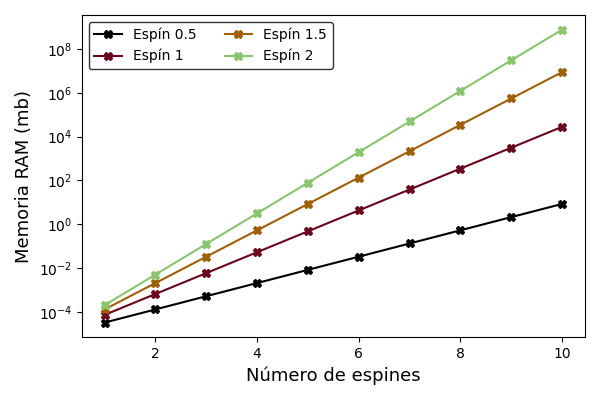
\includegraphics[width=0.7\textwidth]{figures/S1/matriz.png}
\caption{\label{fig:1000} Requerimientos de memoria RAM él para modelo de espines. Fuente: Elaboración propia}
\end{figure}

El segundo problema es que hay que encontrar los elementos necesarios para poder realizar estudios y proyecciones de los efectos derivados de interacciones externas sobre el hamiltoniano. Por ejemplo, para realizar estudios que consideren los efectos de la temperatura, por la descripción matemática del operador de densidad, es necesario tener todos los valores y vectores propios del hamiltoniano. Para hacer esto, es necesario diagonalizar la matriz asociada, lo cual es una tarea computacionalmente costosa cuando el hamiltoniano considera muchas partículas. 


Esta situación presenta un gran obstáculo al momento de realizar investigaciones sobre el comportamiento de la materia, por un lado, si uno desea estudiar sistemas de gran dimensionalidad (muchos cuerpos), se está limitado a trabajar con tipos de hamiltonianos muy concretos que ofrecen una escalabilidad (tamaño de la matriz del modelo) razonable para llevar a cabo una diagonalización exacta, el problema con esto, es que este tipo de hamiltonianos utilizan muchos supuestos, por lo que se puede poner en duda los comportamientos que se pueden derivar de este. Por el otro lado, uno puede realizar estudios exhaustivos (estudios termodinámicos) sobre sistemas de pocos cuerpos, pero lamentablemente, no siempre se puede extrapolar el comportamiento de pocos cuerpos a muchos cuerpos.


\subsection{Estado actual del problema}
Debido a la popularidad de métodos basados en \textit{Density functional theory}, teoría de Hartree-Fock y técnicas basadas en primeros principios, en las últimas décadas se han propuesto diferentes representaciones para tener un uso de recursos más eficiente, además de, crear nuevos métodos con una mejor escalabilidad. Entre ellos, se encuentra la representación MPS/MPO junto al método variacional DRMG que utiliza el concepto de redes tensoriales para representar los sistemas y calcular su estado de mínima energía. Por otro lado, se tienen las aplicaciones de redes neuronales para generar estimadores utilizando resultados, de métodos de \textit{Density functional theory}\cite{Yin2021}, con un bajo error. Las técnicas y métodos mencionados anteriormente corresponden a un paradigma que denominaremos métodos clásicos (que engloban desde métodos exactos hasta métodos variacionales).

En los últimos años, se ha popularizado el uso de computadores cuánticos para realizar simulaciones de sistemas físicos. La computación cuántica no había adquirido esta popularidad porque no existían máquinas cuánticas reales. Desde hace un par de años, Google e IBM anunciaron al público las primeras máquinas cuánticas de pocos \textit{qubits}, las cuales abrieron nuevas posibilidades de aplicaciones y desarrollo en el campo. 

Estas máquinas permiten escapar de la representación matricial, ya que, se trabaja directamente con las funciones de onda que se almacenan en cada \textit{qubits}, por otro lado, se ha demostrado que los algoritmos que se ejecutan en estas máquinas tienen un rendimiento igual o mejor que los algoritmos clásicos (ejemplos de esto es el algoritmo de factorización de números primos de Shor, el algoritmo de Grover entre otros).

Frente a este nuevo paradigma y con los pronósticos de capacidad de las nuevas máquinas, es menester empezar a trabajar en esta área, ya que, al ser un área tan reciente, aún existen muchas aristas en las cuales trabajar (aplicaciones, desarrollo de nuevos métodos, etc.).


\subsection{Objetivos de la solución}
\subsubsection{Objetivo general}
El objetivo general del proyecto es ''Analizar el uso de algoritmos variacionales cuánticos en las simulaciones de estructuras físicas en el contexto de química cuántica y materia condensada''. Este análisis tiene por objetivo visualizar el uso de recursos (de memoria y tiempo) además de contrastar las soluciones obtenidas con los valores exactos.

\subsubsection{Objetivos específicos}
\begin{enumerate}
\item Realizar un estudio que muestre los requerimientos de almacenamiento de los modelos de tipo Fermi-Hubbard, \textit{tight binding}, Heisenberg y estructuras moleculares.
\item Realizar un \textit{benchmark} que contraste los tiempos de ejecución y el error absoluto asociado a la solución obtenida, para el problema de valores y vectores propios, de un algoritmo clásico-exacto, clásico-variacional y variacional cuántico, considerando los modelos expuestos en el punto 1
\item Proponer un diagrama de flujo de trabajo para la utilización algoritmo cuántico, que permita ser generalizado a una amplia gama de hamiltonianos y sistemas de baja dimensión, utilizando rutinas de código abierto y de elaboración propia.
\item Ilustrar la efectividad del diagrama propuesto al aplicarlo en sistemas físicos de baja dimensionalidad.
\end{enumerate}

\subsubsection{Alcance}
Durante el desarrollo del proyecto, se decidió acotarlo en los siguientes aspectos:
\begin{enumerate}
    \item Los parámetros de los modelos se acotaron a regiones y estructuras específicas para limitar el número de posibles combinaciones con los hiperparámetros del \textit{ansatz} y del optimizador (mayor detalle en el capítulo 3).
    \item Por los costos monetarios de uso, se descartó el uso de máquinas cuánticas reales.
\end{enumerate}

